\documentclass{article}

\usepackage{graphicx}
\usepackage{amsmath}
\usepackage{hyperref}
\usepackage{float}
\usepackage{caption}
\usepackage{longtable}


% Bibliography
\usepackage[backend=biber]{biblatex}
\addbibresource{ref.bib}



\title{Meetrapport: Bepaling van de specifieke lading van een elektron}
\author{Koen Kruijt, Hanne Klapwijk}
\date{October 15, 2024}


\begin{document}
\maketitle

Klas: NH2.c \newline
Docent: Triemstra, T.

\newpage
\tableofcontents
\newpage
\section{Doel}
Het doel van de proef is om de specifieke lading van een elektron te bepalen. Dit wordt gedaan door een elektronenbundel in een magnetischveld af te schieten, de elektronen buigen dan af omdat ze geladen zijn. Door de diameter van de bundel en de sterkte van het magnetischveld te meten kan de specifieke lading worden bepaald.
Hier uit volgt ook de onderzoeksvraag: Wat is de specifieke lading van een elektron als deze bepaald word door de straal van de elektronenbaan constant te houden en zowel de spanning op het elektronenkanon, als de stroom op de spoelen te variëren?

\section{Verwachtingen}
De verwachting is dat de waarde van de specifieke lading die gemeten wordt in de buurt komt van de theoretische waarde ($1.76 \times 10^{11} \mathrm{\frac{C}{kg}}$\cite{masscharge}). De gebruikte apparatuur is een "PHYWE: Narrow-beam tube, Pair of Helmholtz coils".

Voor het uitrekenen van de waardes worden de volgende formules gebruikt:
\begin{equation}
	\frac{e}{m} = \frac{2U}{B^2r^2}
	\label{eq:specifiekelading}
\end{equation}
\begin{equation}
	B = 0,715\mu_0 \frac{n \cdot I}{R}
	\label{eq:magnetischveld}
\end{equation}
Waar $\frac{e}{m}$ de specifieke lading is, $U \mathrm{[v]}$ de spanning op het elektronenkanon, $B \mathrm{[T]}$ de magnetische veldsterkte, $r \mathrm{[m]}$ de straal van de elektronenbundel, $\mu_0 \mathrm{[N\cdot A^{-2}]}$ de magnetische permeabiliteit, $n \mathrm{[1]}$ het aantal windingen van de spoel, $I \mathrm{[A]}$ de stroomsterkte door de spoel en $R \mathrm{[m]}$ de straal van de spoelen.

Uit \ref{eq:specifiekelading} volgt de volgende linearisatie:
\begin{equation}
	U =\frac{e}{m} \cdot B^2 \cdot r^2 \cdot \frac{1}{2}
	\label{eq:linearisatie}
\end{equation}
Die gebruikt kan worden om de specifieke lading te bepalen door middel het aflezen van de richtingscoëfficiënt.

En de verwachting is dus een mooie rechte lijn te zien in de grafiek van $U$ tegen $\frac{1}{2}B^2\cdot r^2$ zoals in \ref{eq:linearisatie} beschreven is.

\section{Schematische weergave van de opstelling}

\begin{figure}[H]
	\centering
	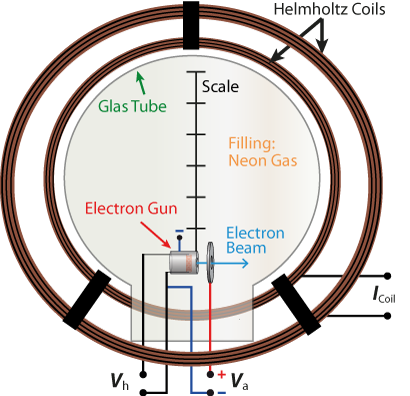
\includegraphics[width=0.7\textwidth]{opstelling.png}
	\caption{De opstelling van de proef; Naar \cite{schematic}}
	\label{fig:opstelling}
\end{figure}
De elektronenbundel gaat met de richting van het pijltje in \ref{fig:opstelling} mee en wordt circulair afgebogen door het magnetisch veld van de spoelen. De bundel gaat door een ladder met sporten op bekende afstand van elkaar, zo kan de diameter van de bundel worden bepaald. De spanning en de stroomsterkte worden gemeten met een multimeter.
Het maat plan volgt:
\begin{enumerate}
	\item Aansluiten aan de voedingen en meters
	\item Kies een sport op de ladder uit
	\item Zorg dat de elektronenbundel op de sport valt
	\item Verander de stroomsterkte (dus bundel valt niet op de gekozen sport)
	\item Verander spanning tot de bundel weer op de sport valt
	\item Noteer en herhaal voor meet reeks, en verander de sport
\end{enumerate}

\section{Resultaten}

%plot.png
\begin{figure}[H]
	\centering
	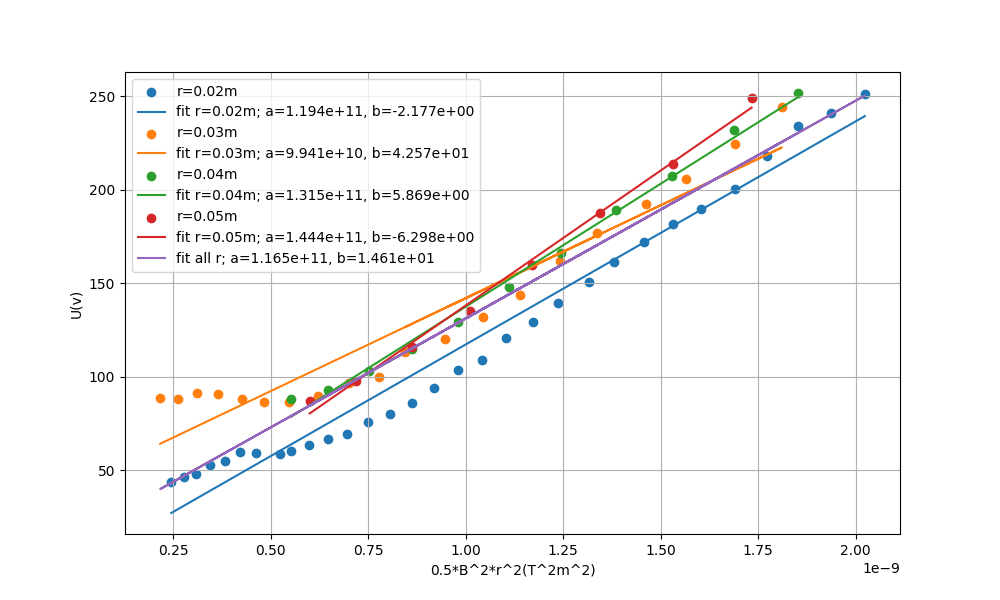
\includegraphics[width=1\textwidth]{plot.png}
	\caption{De gemeten waardes van de spanning en de magnetische veldsterkte}
	\label{fig:plot}
\end{figure}
In \ref{fig:plot} heeft de fit de volgende coefficienten $a=1,165 \cdot 10^{11}\pm 4,262 \cdot 10^{9}, b=1,461 \cdot 10^{1}\pm 4,773 \cdot 10^{0}$, hieruit volgt dat de gemeten specifieke lading van een elektron $1,165 \cdot 10^{11} \mathrm{\frac{C}{kg}}$ is, dit is natuurlijk erg afwijkend.


\section{Uitwerking \& discussie}
De gemeten waarde van de specifieke lading van een elektron is $1,165 \cdot 10^{11} \mathrm{\frac{C}{kg}}$, dit is erg afwijkend van de theoretische waarde van $1,76 \cdot 10^{11} \mathrm{\frac{C}{kg}}$. Dit komt hoogst waarschijnlijk door een afwijkende veld sterkte van de berekende waarde en een kleine afwijking in de afstand tussen de sporten in.


\section{Conclusie}
De conclusie van deze proef is dat de onderzoeksvraag niet beantwoord is, dit komt omdat de meting erg sensitief is voor afwijkingen in het B veld en dit niet direct te meten was met de gebruikte apparatuur, en dus niet mogelijk om hier voor te compenseren. 

\nocite{*}
\printbibliography[title={Referenties}]


\section{Bijlagen}

%\begin{table}
    \centering
    \begin{longtable}{|l|l|l|l|}
    \hline
        I & U & B & Br \\ \hline
        2 cm & ~ & ~ & ~ \\ \hline
        1.601 & 43.6863 & 0.001107077 & 2.45124E-10 \\ \hline
        1.702 & 46.271 & 0.001176917 & 2.77027E-10 \\ \hline
        1.797 & 48.0852 & 0.001242609 & 3.08815E-10 \\ \hline
        1.9 & 52.553 & 0.001313833 & 3.45231E-10 \\ \hline
        2.001 & 54.868 & 0.001383673 & 3.8291E-10 \\ \hline
        2.102 & 59.742 & 0.001453514 & 4.2254E-10 \\ \hline
        2.202 & 59.268 & 0.001522663 & 4.637E-10 \\ \hline
        2.34 & 58.835 & 0.001618088 & 5.23642E-10 \\ \hline
        2.401 & 60.162 & 0.001660269 & 5.51299E-10 \\ \hline
        2.502 & 63.728 & 0.00173011 & 5.98656E-10 \\ \hline
        2.601 & 66.423 & 0.001798568 & 6.46969E-10 \\ \hline
        2.699 & 69.501 & 0.001866334 & 6.9664E-10 \\ \hline
        2.802 & 75.884 & 0.001937557 & 7.50826E-10 \\ \hline
        2.903 & 80.004 & 0.002007398 & 8.05929E-10 \\ \hline
        3.004 & 86.056 & 0.002077238 & 8.62984E-10 \\ \hline
        3.101 & 94.025 & 0.002144313 & 9.19616E-10 \\ \hline
        3.202 & 103.702 & 0.002214154 & 9.80495E-10 \\ \hline
        3.301 & 108.666 & 0.002282611 & 1.04206E-09 \\ \hline
        3.397 & 120.547 & 0.002348994 & 1.10355E-09 \\ \hline
        3.501 & 129.481 & 0.002420909 & 1.17216E-09 \\ \hline
        3.598 & 139.277 & 0.002487984 & 1.23801E-09 \\ \hline
        3.709 & 150.86 & 0.002564739 & 1.31558E-09 \\ \hline
        3.801 & 161.538 & 0.002628357 & 1.38165E-09 \\ \hline
        3.905 & 171.92 & 0.002700272 & 1.45829E-09 \\ \hline
        4.002 & 181.54 & 0.002767346 & 1.53164E-09 \\ \hline
        4.096 & 189.783 & 0.002832346 & 1.60444E-09 \\ \hline
        4.206 & 200.583 & 0.00290841 & 1.69177E-09 \\ \hline
        4.305 & 218.255 & 0.002976868 & 1.77235E-09 \\ \hline
        4.402 & 234.067 & 0.003043943 & 1.85312E-09 \\ \hline
        4.5 & 241.285 & 0.003111709 & 1.93655E-09 \\ \hline
        4.6 & 251.491 & 0.003180858 & 2.02357E-09 \\ \hline
        3 cm & ~ & ~ & ~ \\ \hline
        1.982 & 112.987 & 0.001370535 & 8.45264E-10 \\ \hline
        2.492 & 176.82 & 0.001723195 & 1.33623E-09 \\ \hline
        2.099 & 120.431 & 0.001451439 & 9.48004E-10 \\ \hline
        2.203 & 131.847 & 0.001523354 & 1.04427E-09 \\ \hline
        2.301 & 143.758 & 0.00159112 & 1.13925E-09 \\ \hline
        2.402 & 161.627 & 0.001660961 & 1.24146E-09 \\ \hline
        2.607 & 192.618 & 0.001802717 & 1.4624E-09 \\ \hline
        2.697 & 205.872 & 0.001864951 & 1.56512E-09 \\ \hline
        2.803 & 224.296 & 0.001938249 & 1.69056E-09 \\ \hline
        2.901 & 244.334 & 0.002006015 & 1.81084E-09 \\ \hline
        1.901 & 99.709 & 0.001314524 & 7.77588E-10 \\ \hline
        1.805 & 96.665 & 0.001248141 & 7.01035E-10 \\ \hline
        1.701 & 89.728 & 0.001176226 & 6.22578E-10 \\ \hline
        1.594 & 86.484 & 0.001102236 & 5.46716E-10 \\ \hline
        1.497 & 86.565 & 0.001035162 & 4.82202E-10 \\ \hline
        1.406 & 87,910 & 0.000972236 & 4.25359E-10 \\ \hline
        1.301 & 90.881 & 0.00089963 & 3.642E-10 \\ \hline
        1.203 & 91.164 & 0.000831863 & 3.11399E-10 \\ \hline
        1.103 & 88.021 & 0.000762714 & 2.6178E-10 \\ \hline
        1.004 & 88.627 & 0.000694257 & 2.16897E-10 \\ \hline
        4 cm & ~ & ~ & ~ \\ \hline
        1.201 & 88.156 & 0.00083048 & 5.51758E-10 \\ \hline
        1.301 & 92.971 & 0.00089963 & 6.47467E-10 \\ \hline
        1.402 & 103.177 & 0.00096947 & 7.51898E-10 \\ \hline
        1.502 & 114.612 & 0.001038619 & 8.62984E-10 \\ \hline
        1.601 & 129.5 & 0.001107077 & 9.80495E-10 \\ \hline
        1.705 & 148.227 & 0.001178992 & 1.11202E-09 \\ \hline
        1.803 & 166.013 & 0.001246758 & 1.24352E-09 \\ \hline
        1.904 & 189.26 & 0.001316598 & 1.38675E-09 \\ \hline
        2 & 207.319 & 0.001382982 & 1.53011E-09 \\ \hline
        2.1 & 231.959 & 0.001452131 & 1.68695E-09 \\ \hline
        2.201 & 251.762 & 0.001521971 & 1.85312E-09 \\ \hline
        5 cm & ~ & ~ & ~ \\ \hline
        1.002 & 86.819 & 0.000692874 & 6.00093E-10 \\ \hline
        1.0977 & 97.642 & 0.000759049 & 7.20195E-10 \\ \hline
        1.202 & 115.966 & 0.000831172 & 8.63558E-10 \\ \hline
        1.301 & 135.37 & 0.00089963 & 1.01167E-09 \\ \hline
        1.4 & 159.887 & 0.000968087 & 1.17149E-09 \\ \hline
        1.5 & 187.415 & 0.001037236 & 1.34482E-09 \\ \hline
        1.601 & 213.647 & 0.001107077 & 1.53202E-09 \\ \hline
        1.703 & 248.875 & 0.001177609 & 1.73345E-09 \\ \hline
    \end{longtable}
%\end{table}



\end{document}